% -------------------------------------------------------
% Secção 3 – Arquitetura e Demonstrador
% -------------------------------------------------------

% -------------------------------------------------------
\subsection*{3.1 Visão Geral da Arquitetura}
\addcontentsline{toc}{subsection}{3.1 Visão Geral da Arquitetura}

O sistema implementa o modelo X/Open DTP com cinco tipos de elemento serviço, cujas
responsabilidades estão sintetizadas na Tabela~\ref{tab:servicos}. A comunicação entre
serviços é inteiramente via \textbf{gRPC sobre plain-text}, com contratos formalizados em
ficheiros \texttt{.proto}. Cada serviço é encapsulado num contentor \textbf{Podman},
com portas gRPC atribuídas estaticamente: \texttt{Service.Vector} nas portas 9000 e 9001,
\texttt{Service.TM} na porta 9002, e \texttt{Service.TPLM} na porta 9003.

\begin{table}[ht]
\centering
\begin{tabularx}{\textwidth}{llX}
\toprule
\textbf{Serviço} & \textbf{Papel X/Open} & \textbf{Descrição} \\
\midrule
\texttt{Service.Vector} ($M$ instâncias) & Resource Manager (RM) &
  Gere um vetor de $N$ inteiros; expõe operações transacionais XA via gRPC \\
\texttt{Service.Client} ($K$ instâncias) & Application Program (AP) &
  Executa transferências concorrentes entre vetores \\
\texttt{Service.TM}                      & Transaction Manager (TM) &
  Fachada transacional e coordenador do protocolo 2PC \\
\texttt{Service.TPLM}                    & Gestor de Concorrência &
  Gere locks 2PL; deteção de deadlock por grafo wait-for \\
\texttt{Service.Validator}               & Application Program (AP) &
  Verifica transacionalmente o invariante $\sum$ vetores \\
\bottomrule
\end{tabularx}
\caption{Elementos serviço do sistema e mapeamento ao modelo X/Open DTP.}
\label{tab:servicos}
\end{table}

Uma decisão arquitetural relevante do demonstrador é o papel do \texttt{Service.TM} como
\textbf{fachada total}: o \texttt{Service.Client} não contacta diretamente os vetores nem o
TPLM --- todas as operações de leitura, escrita e gestão de locks são mediadas pelo TM. Isto
simplifica o cliente mas centraliza no TM a coordenação de concorrência e dados, afastando-se
do modelo X/Open canónico, em que o AP comunica diretamente com os RMs e apenas delega a
coordenação 2PC ao TM. A Figura~\ref{fig:architecture} sintetiza as dependências de
comunicação.

\begin{figure}[ht]
\centering
\begin{tikzpicture}[
  node distance=1.5cm and 2.8cm,
  box/.style={rectangle, draw, rounded corners, minimum width=2.8cm,
              minimum height=0.9cm, align=center, font=\small},
  arr/.style={->, >=stealth, thick},
  arrd/.style={->, >=stealth, thick, dashed, gray}
]

\node[box, fill=blue!15]   (client)    {Service.Client\\(AP)};
\node[box, fill=green!15,  right=3.2cm of client]          (tm)     {Service.TM\\(TM) :9002};
\node[box, fill=orange!15, above right=0.8cm and 2.6cm of tm] (vec1) {Service.Vector\\(RM) :9000};
\node[box, fill=orange!15, below right=0.8cm and 2.6cm of tm] (vec2) {Service.Vector\\(RM) :9001};
\node[box, fill=red!15,    below=2.0cm of tm]              (tplm)   {Service.TPLM\\:9003};
\node[box, fill=gray!10,   below=1.4cm of tplm]            (zk)     {ZooKeeper\\(3 nós)};
\node[box, fill=blue!8,    below=0.6cm of client]          (val)    {Service.Validator\\\small\textit{[TODO: implementar]}};

\draw[arr]  (client) -- node[above, font=\scriptsize]{begin/read/write/commit} (tm);
\draw[arr]  (tm) -- node[above left,  font=\scriptsize]{prepareWrite/commit/abort} (vec1);
\draw[arr]  (tm) -- node[below left,  font=\scriptsize]{prepareWrite/commit/abort} (vec2);
\draw[arr]  (tm) -- node[right,       font=\scriptsize]{acquireLock/releaseLocks}  (tplm);
\draw[arr]  (tplm) -- node[right,     font=\scriptsize]{eleição de líder}          (zk);
\draw[arr]  (tm.south east) to[out=-20, in=40, looseness=2.0]
            node[right, font=\scriptsize, pos=0.45]{eleição / descobre TPLM}       (zk.east);
\draw[arrd] (val)  -- node[below,     font=\scriptsize]{begin/read/commit}         (tm);

\end{tikzpicture}
\caption{Diagrama de arquitetura do sistema. Ligação a tracejado indica o
  \texttt{Service.Validator}, ainda não implementado. O ZooKeeper está integrado em
  \texttt{Service.TPLM} e \texttt{Service.TM} para eleição de líder e descoberta dinâmica
  de endereços.}
\label{fig:architecture}
\end{figure}
\FloatBarrier

% -------------------------------------------------------
\subsection*{3.2 Estratégia e Implementação}
\addcontentsline{toc}{subsection}{3.2 Estratégia e Implementação}

A \textbf{stack tecnológica} adotada é Java 21 com Quarkus como framework de microserviços,
gRPC com Protobuf 3 como protocolo de comunicação, e Podman para containerização. O Quarkus
oferece suporte nativo a gRPC via a extensão \texttt{quarkus-grpc}, integrando automaticamente
os stubs gerados pelo \texttt{protoc} no ciclo de vida CDI. O modelo reactivo Mutiny (API
\texttt{Uni<T>}) é utilizado para as chamadas gRPC, com anotação \texttt{@Blocking} nas
operações que adquirem locks (impedindo o bloqueio do event-loop reactivo). Esta decisão é
particularmente relevante no \texttt{Service.TPLM}, onde as operações de aquisição de lock
podem ficar em espera por longos períodos.

Esta stack poderia facilmente ser substituída por \textbf{implementações em outras linguagens}
--- Python (\texttt{grpcio}), C\#/.NET (\texttt{Grpc.AspNetCore}), ou Go
(\texttt{google.golang.org/grpc}) --- pois os contratos \texttt{.proto} são independentes da
linguagem de implementação. O compilador \texttt{protoc} gera stubs para cada ecossistema a
partir do mesmo ficheiro de contrato, garantindo que um cliente Java pode invocar um
\texttt{Service.Vector} em Python sem qualquer adaptação adicional, desde que ambos respeitem
o mesmo \texttt{.proto}. No contexto empresarial, esta propriedade viabiliza o desenvolvimento
paralelo por equipas com culturas tecnológicas distintas, como discutido na Secção~2.4.

O desenvolvimento de um sistema com cinco tipos de elemento serviço interdependentes impôs
dificuldades concretas que vão além da complexidade teórica. A coordenação de arranque
(ZooKeeper $\to$ TPLM $\to$ TM $\to$ Vector(es) $\to$ Cliente) exige sincronização cuidadosa:
um TM que arranque antes do TPLM estar disponível falha a primeira tentativa de aquisição de
lock. A ausência de um service registry (Consul) obriga à configuração estática de endereços
via variáveis de ambiente e ficheiros \texttt{application.properties}, tornando a reconfiguração
operacionalmente rígida. Cada nova instância de \texttt{Service.Vector} exige atualização manual
da configuração do TM. Estas fricções, embora gerenciáveis num demonstrador de dimensão fixa,
tornar-se-iam intratáveis em produção, ilustrando concretamente as dificuldades discutidas na
Secção~2.2.

\subsubsection*{Service.Vector (Resource Manager)}

O \texttt{Service.Vector} implementa a interface RM do modelo X/Open, expondo operações
transacionais através do contrato Protobuf seguinte:

\begin{lstlisting}[language=proto, caption={Contrato gRPC do \texttt{Service.Vector} (Dvector.proto).}]
service DvectorService {
  rpc Read          (ReadRequest)  returns (ReadResponse);
  rpc PrepareWrite  (WriteRequest) returns (AckResponse);
  rpc Commit        (TxRequest)    returns (AckResponse);
  rpc Abort         (TxRequest)    returns (AckResponse);
  rpc SumVector     (Empty)        returns (SumResponse);
  rpc InvariantCheck(Empty)        returns (AckResponse);
}

message WriteRequest {
  string tx_id = 1;
  int32  pos   = 2;
  int32  value = 3;
}
\end{lstlisting}

A semântica XA é implementada através de uma \textbf{área de staging por transação}:
\texttt{PrepareWrite} armazena a escrita temporariamente num \texttt{ConcurrentHashMap}
indexado por \texttt{txId}, sem alterar o vetor persistente. \texttt{Commit} aplica as
escritas staged ao vetor sob \texttt{synchronized(vector)}, garantindo atomicidade local.
\texttt{Abort} descarta a entrada do staging sem nenhuma alteração ao estado persistente.
O excerto seguinte ilustra esta mecânica:

\begin{lstlisting}[language=Java, caption={Área de staging e commit no \texttt{DvectorImpl} (excerto).}]
private static final List<Integer> vector = Arrays.asList(300, 234, 56, 789);
private static final Map<String, Map<Integer, Integer>> pendingWrites =
        new ConcurrentHashMap<>();

@Override
public Uni<AckResponse> prepareWrite(WriteRequest request) {
    pendingWrites
        .computeIfAbsent(request.getTxId(), k -> new ConcurrentHashMap<>())
        .put(request.getPos(), request.getValue());
    return Uni.createFrom().item(
        AckResponse.newBuilder().setMessage(request.getTxId()).build());
}

@Override
public Uni<AckResponse> commit(TxRequest request) {
    Map<Integer, Integer> writes = pendingWrites.remove(request.getTxId());
    if (writes != null) {
        synchronized (vector) {
            writes.forEach(vector::set);
        }
    }
    return Uni.createFrom().item(/* ... */);
}
\end{lstlisting}

O demonstrador inicializa cada instância de \texttt{Service.Vector} com o vetor fixo
\texttt{[300, 234, 56, 789]} (soma = 1379), servindo como valor inicial do invariante.

\subsubsection*{Service.TPLM (Two-Phase Lock Manager)}

O \texttt{Service.TPLM} implementa o coordenador de concorrência 2PL, expondo o
seguinte contrato:

\begin{lstlisting}[language=proto, caption={Contrato gRPC do \texttt{Service.TPLM} (tplm.proto).}]
service TplmService {
  rpc AcquireLock   (LockRequest) returns (LockResponse);
  rpc ReleaseAllLocks(TxRequest)  returns (LockResponse);
  rpc CheckLock     (LockRequest) returns (LockResponse);
  rpc GetLockTable  (Empty)       returns (LockTableResponse);
}

message LockRequest {
  string tx_id      = 1;
  string service_id = 2;  // identificador do vector
  int32  pos        = 3;  // posição no vector
}
\end{lstlisting}

A implementação mantém em memória três estruturas principais: \texttt{lockTable}
(\texttt{Map\textless String, LockEntry\textgreater}), indexada pela chave composta
\texttt{serviceId:pos} que representa cada par \texttt{(vecId,~index)} como recurso
independente, alinhado com a granularidade confirmada pelo professor (OBS-04);
\texttt{txHeldLocks} (\texttt{Map\textless String, Set\textless String\textgreater\textgreater}),
que regista o conjunto de recursos bloqueados por cada transação activa, permitindo a
libertação eficiente em \texttt{releaseAllLocks}; e \texttt{waitForGraph}
(\texttt{Map\textless String, String\textgreater}), utilizado na deteção de deadlock por
ciclo. A sincronização é garantida por um \texttt{ReentrantLock(true)} global
(\texttt{globalMutex}), que assegura equidade (\textit{fair scheduling}) na ordem de
atribuição de locks. O timeout de espera é de 5\,segundos, após o qual a operação retorna
\texttt{TIMEOUT} e a transação solicitante é responsável pelo seu próprio abort.

\begin{lstlisting}[language=Java, caption={Granularidade de lock por \texttt{(vecId,~index)} no \texttt{TwoPhaseLockManagerImpl}.}]
private static String resourceKey(String serviceId, int pos) {
    return serviceId + ":" + pos;
}
\end{lstlisting}

Com esta granularidade, duas transações que acedam a posições distintas do mesmo vetor
(e.g., \texttt{CSerDvector01[0]} e \texttt{CSerDvector01[2]}) não entram em conflito e
progridem em paralelo, reduzindo a contenção face a uma granularidade por vetor inteiro.

\textbf{Limitação: ausência de tipos de lock.}
A implementação atual não distingue entre \textbf{ReadLock} (partilhado) e
\textbf{WriteLock} (exclusivo) --- todos os locks são tratados como exclusivos,
representados por um único campo \texttt{holder} por entrada da \texttt{lockTable}. Dois
leitores concorrentes do mesmo elemento bloqueiam-se mutuamente, contrariando a semântica
do 2PL apresentada na Secção~2.1 (read-read compatível). O impacto é uma contenção
adicional nas operações de leitura --- em particular durante a verificação do invariante
pelo \texttt{Service.Validator}, que emite read locks em todos os elementos antes de somar.

Para alta disponibilidade, o \texttt{Service.TPLM} integra o módulo partilhado
\texttt{ZooKeeperLIB} via a classe \texttt{ZkRegistrar}, que inicia uma eleição de líder
ZooKeeper no arranque do serviço. O mecanismo é descrito em detalhe na Secção~3.4.

\subsubsection*{Service.TM (Transaction Manager)}

O \texttt{Service.TM} expõe ao cliente operações de ciclo de vida de transação e de
leitura/escrita mediadas, assumindo o papel de fachada total:

\begin{lstlisting}[language=proto, caption={Contrato gRPC do \texttt{Service.TM} (Tm.proto).}]
service TmService {
  rpc BeginTransaction(BeginRequest)  returns (TxResponse);
  rpc Read            (ReadRequest)   returns (ReadResponse);
  rpc Write           (WriteRequest)  returns (TxResponse);
  rpc Commit          (TxRequest)     returns (TxResponse);
  rpc Abort           (TxRequest)     returns (TxResponse);
  rpc GetTransactions (GetTxRequest)  returns (TxResponse);
}

message ReadRequest {
  string tx_id     = 1;
  string vector_id = 2;
  int32  pos       = 3;
}
\end{lstlisting}

O TM mantém um registo em memória das transações ativas (\texttt{Map\textless String,
TxRecord\textgreater}), cada uma com o seu estado (\texttt{ACTIVE}, \texttt{PREPARING},
\texttt{COMMITTED}, \texttt{ABORTED}) e a lista de RMs participantes.

A \textbf{resolução de endereços} dos vectores é feita por prioridade: primeiro via
propriedade de configuração \texttt{vector.address.\{id\}}, depois via variável de ambiente
\texttt{\{ID\}\_GRPC\_TARGET}, com fallback para \texttt{localhost:9000}. Esta abordagem
substitui funcionalmente o Consul (não implementado), limitando a flexibilidade operacional
mas simplificando o setup.

\textbf{Descoberta do TPLM activo via ZooKeeper.}
Em vez de um endereço estático, o \texttt{TransactionManagerImpl} resolve dinamicamente o
\texttt{Service.TPLM} activo antes de cada chamada gRPC, invocando
\texttt{ZkLeaderElection.resolveLeaderAddress()}, que lê o z-node \texttt{/tplm/leader}
onde o TPLM líder publica o seu endereço. Se o ZooKeeper estiver inacessível, é utilizado
o endereço configurado em \texttt{tplm.grpc.target} como fallback. O TM possui igualmente
um \texttt{ZkRegistrar} próprio com path \texttt{/tm}, tornando-o elegível para operação
em modo ativo-passivo: múltiplas instâncias do TM participam na eleição, e o
\texttt{Service.Client} descobre o TM activo lendo \texttt{/tm/leader} --- ver
Secção~3.4 para o mecanismo completo.

O protocolo \textbf{2PC implementado} diverge ligeiramente do modelo canónico. Na Fase~1,
em vez de uma operação \texttt{xa\_prepare()} explícita, o TM chama \texttt{SumVector()} em
cada RM como sonda de disponibilidade (\textit{health-check}). A semântica de prepare ---
garantir que o RM persiste o estado staged antes de votar --- é assegurada implicitamente
pelo facto de \texttt{PrepareWrite} já ter armazenado as escritas no staging a montante. Na
Fase~2, o TM chama \texttt{Commit(txId)} em cada RM para aplicar as escritas staged, seguido
de \texttt{ReleaseAllLocks(txId)} no TPLM:

\begin{lstlisting}[language=Java, caption={Implementação do 2PC no \texttt{TransactionManagerImpl} (excerto).}]
@Override
public String commit(String txId) {
    TxRecord tx = requireActiveTx(txId);
    tx.state = TxState.PREPARING;

    // Fase 1: sonda de disponibilidade (health-check por sumVector)
    List<String> failedServices = new ArrayList<>();
    for (Map.Entry<String, String> vector : tx.enlistedVectors.entrySet()) {
        try {
            buildDvectorClient(vector.getValue()).sumVector();
        } catch (Exception e) {
            failedServices.add(vector.getKey());
        }
    }
    if (!failedServices.isEmpty())
        return abortAndReleaseLocks(txId, tx, "prepare-failed:" + failedServices);

    // Fase 2: commit em todos os RMs
    for (Map.Entry<String, String> vector : tx.enlistedVectors.entrySet()) {
        buildDvectorClient(vector.getValue()).commit(txId);
    }
    releaseLocks(txId);          // liberta locks no TPLM
    tx.state = TxState.COMMITTED;
    return "COMMITTED";
}
\end{lstlisting}

Uma \textbf{limitação relevante} é a ausência de log de transações persistente: o estado do
TM é mantido exclusivamente em memória. Em caso de falha do TM após completar a Fase~1 mas
antes de concluir a Fase~2, os RMs participantes ficam bloqueados em estado
\textit{in-doubt} com as escritas staged e os locks detidos, sem possibilidade de recuperação
automática. Esta limitação é reconhecida como trabalho futuro; o modelo X/Open exige que o
TM registe a decisão de commit em armazenamento estável antes de iniciar a Fase~2
(\textit{write-ahead log}).

\subsubsection*{Service.Client (Application Program)}

O \texttt{Service.Client} implementa o papel de AP transacional, comunicando
exclusivamente com o \texttt{Service.TM}. O ciclo de execução compreende três fases:

\begin{enumerate}[label=\alph*)]
  \item \textbf{Transferências intra-vetor} (2 iterações por default, configurável via
        \texttt{client.transfer.iterations}): transferência de \texttt{amount} unidades
        entre as posições 0 e 2 do mesmo vetor (\texttt{CSerDvector01}), demonstrando a
        serializabilidade de acessos concorrentes a um único RM.
  \item \textbf{Transferência inter-vetores}: transferência entre posição~0 de
        \texttt{CSerDvector01} e posição~0 de \texttt{CSerDvector02}, envolvendo dois RMs
        participantes no mesmo 2PC.
  \item \textbf{Verificação do invariante}: leitura transacional de todas as posições de
        ambos os vetores via TM, seguida de commit. O cliente verifica que a soma total
        corresponde a $2 \times 1379 = 2758$.
\end{enumerate}

Em caso de conflito de locks (\texttt{DEADLOCK} ou \texttt{TIMEOUT} devolvidos pelo TPLM
como exceção no TM), o cliente efetua abort e retenta até 5 vezes com um intervalo de 150\,ms,
após o qual desiste e regista a transação como abortada.

O \texttt{Service.Client} descobre dinamicamente o \texttt{Service.TM} activo através de
\texttt{ZkLeaderElection.resolveLeaderAddress()}, que lê o z-node \texttt{/tm/leader} antes
de cada chamada gRPC ao TM. Se o ZooKeeper estiver inacessível, é utilizado o endereço
configurado em \texttt{tm.grpc.target} como fallback (\texttt{zk.enabled=false}).

\subsubsection*{Service.Validator (Application Program — não implementado)}

\begin{quote}
\textit{\textbf{TODO:} O \texttt{Service.Validator} não se encontra implementado no demonstrador
atual. A sua função, descrita em detalhe na Secção~2.1, é verificar o invariante
$\sum_i \text{sum}(\text{vector}_i) = K$ operando como AP transacional --- adquirindo
ReadLocks em todos os pares \texttt{(vecId,~index)} antes de calcular o somatório, de modo a
garantir uma leitura serializada. Este componente deve ser invocado nos três momentos definidos
no plano: antes de qualquer transação de cliente (verificação de sanidade), após
\texttt{xa\_commit} bem-sucedido em todos os RMs, e após \texttt{xa\_rollback} bem-sucedido em
todos os RMs. A sua ausência não compromete a correção do demonstrador para os casos de teste
atuais, mas impede a validação automatizada do invariante após cada transação.}
\end{quote}

% -------------------------------------------------------
\subsection*{3.3 Fluxo Completo de uma Transação}
\addcontentsline{toc}{subsection}{3.3 Fluxo Completo de uma Transação}

O diagrama de sequência seguinte ilustra o fluxo completo de uma transferência
inter-vetores no demonstrador implementado (dois RMs: \texttt{CSerDvector01} e
\texttt{CSerDvector02}). A sequência reflete a arquitetura de fachada do TM:

\begin{figure}[ht]
\centering
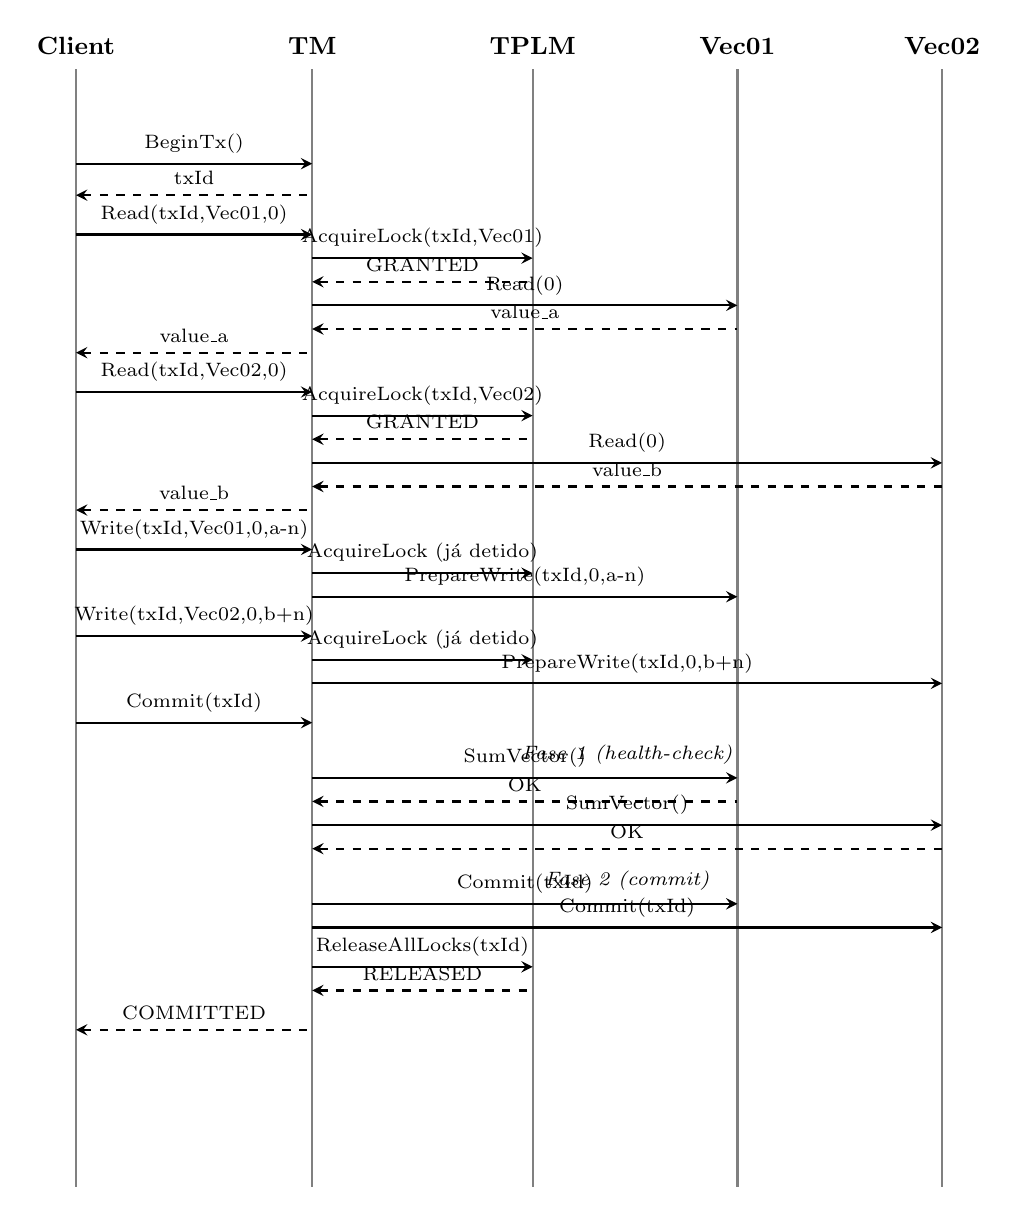
\begin{tikzpicture}[
  font=\small,
  lifeline/.style={thick, gray},
  msg/.style={->, >=stealth, thick},
  retmsg/.style={<-, >=stealth, thick, dashed},
  lbl/.style={font=\scriptsize, midway, above, sloped}
]

% Lifeline positions (x)
\def\xCli{0}
\def\xTM{3}
\def\xTPLM{5.8}
\def\xVA{8.4}
\def\xVB{11.0}

% Header labels
\node[align=center] at (\xCli, 1.0)  {\textbf{Client}};
\node[align=center] at (\xTM,  1.0)  {\textbf{TM}};
\node[align=center] at (\xTPLM,1.0)  {\textbf{TPLM}};
\node[align=center] at (\xVA,  1.0)  {\textbf{Vec01}};
\node[align=center] at (\xVB,  1.0)  {\textbf{Vec02}};

% Lifelines
\foreach \x in {\xCli,\xTM,\xTPLM,\xVA,\xVB} {
  \draw[lifeline] (\x,0.7) -- (\x,-13.5);
}

% Messages (y decreasing = time progressing)
% 1. BeginTransaction
\draw[msg] (\xCli,-0.5) -- node[lbl]{BeginTx()} (\xTM,-0.5);
\draw[retmsg] (\xCli,-0.9) -- node[lbl]{txId} (\xTM,-0.9);

% 2. Read Vec01[0]
\draw[msg] (\xCli,-1.4) -- node[lbl]{Read(txId,Vec01,0)} (\xTM,-1.4);
\draw[msg] (\xTM,-1.7) -- node[lbl]{AcquireLock(txId,Vec01)} (\xTPLM,-1.7);
\draw[retmsg] (\xTM,-2.0) -- node[lbl]{GRANTED} (\xTPLM,-2.0);
\draw[msg] (\xTM,-2.3) -- node[lbl]{Read(0)} (\xVA,-2.3);
\draw[retmsg] (\xTM,-2.6) -- node[lbl]{value\_a} (\xVA,-2.6);
\draw[retmsg] (\xCli,-2.9) -- node[lbl]{value\_a} (\xTM,-2.9);

% 3. Read Vec02[0]
\draw[msg] (\xCli,-3.4) -- node[lbl]{Read(txId,Vec02,0)} (\xTM,-3.4);
\draw[msg] (\xTM,-3.7) -- node[lbl]{AcquireLock(txId,Vec02)} (\xTPLM,-3.7);
\draw[retmsg] (\xTM,-4.0) -- node[lbl]{GRANTED} (\xTPLM,-4.0);
\draw[msg] (\xTM,-4.3) -- node[lbl]{Read(0)} (\xVB,-4.3);
\draw[retmsg] (\xTM,-4.6) -- node[lbl]{value\_b} (\xVB,-4.6);
\draw[retmsg] (\xCli,-4.9) -- node[lbl]{value\_b} (\xTM,-4.9);

% 4. Write Vec01
\draw[msg] (\xCli,-5.4) -- node[lbl]{Write(txId,Vec01,0,a-n)} (\xTM,-5.4);
\draw[msg] (\xTM,-5.7) -- node[lbl]{AcquireLock (já detido)} (\xTPLM,-5.7);
\draw[msg] (\xTM,-6.0) -- node[lbl]{PrepareWrite(txId,0,a-n)} (\xVA,-6.0);

% 5. Write Vec02
\draw[msg] (\xCli,-6.5) -- node[lbl]{Write(txId,Vec02,0,b+n)} (\xTM,-6.5);
\draw[msg] (\xTM,-6.8) -- node[lbl]{AcquireLock (já detido)} (\xTPLM,-6.8);
\draw[msg] (\xTM,-7.1) -- node[lbl]{PrepareWrite(txId,0,b+n)} (\xVB,-7.1);

% 6. Commit
\draw[msg] (\xCli,-7.6) -- node[lbl]{Commit(txId)} (\xTM,-7.6);

% 2PC Phase 1
\node[font=\scriptsize\itshape] at (7.0,-8.0) {Fase 1 (health-check)};
\draw[msg] (\xTM,-8.3) -- node[lbl]{SumVector()} (\xVA,-8.3);
\draw[retmsg] (\xTM,-8.6) -- node[lbl]{OK} (\xVA,-8.6);
\draw[msg] (\xTM,-8.9) -- node[lbl]{SumVector()} (\xVB,-8.9);
\draw[retmsg] (\xTM,-9.2) -- node[lbl]{OK} (\xVB,-9.2);

% 2PC Phase 2
\node[font=\scriptsize\itshape] at (7.0,-9.6) {Fase 2 (commit)};
\draw[msg] (\xTM,-9.9) -- node[lbl]{Commit(txId)} (\xVA,-9.9);
\draw[msg] (\xTM,-10.2) -- node[lbl]{Commit(txId)} (\xVB,-10.2);

% Release locks
\draw[msg] (\xTM,-10.7) -- node[lbl]{ReleaseAllLocks(txId)} (\xTPLM,-10.7);
\draw[retmsg] (\xTM,-11.0) -- node[lbl]{RELEASED} (\xTPLM,-11.0);

% Return to client
\draw[retmsg] (\xCli,-11.5) -- node[lbl]{COMMITTED} (\xTM,-11.5);

\end{tikzpicture}
\caption{Diagrama de sequência de uma transferência inter-vetores ($n$ unidades de
  \texttt{Vec01[0]} para \texttt{Vec02[0]}). O TM atua como fachada: todas as
  operações de leitura, escrita e lock são mediadas pelo TM.}
\label{fig:sequence}
\end{figure}
\FloatBarrier

O diagrama evidencia uma propriedade importante da arquitetura de fachada: cada operação
\texttt{Read} e \texttt{Write} do cliente resulta em dois round-trips de rede internos ao TM
(um para o TPLM e um para o vetor), duplicando a latência de coordenação face a uma arquitetura
em que o cliente contactaria diretamente os RMs.
O custo por transação inter-vetores é de \textbf{12 round-trips gRPC} (4 leituras/escritas
$\times$ 2 + 4 fases do 2PC + 2 releaseLocks), comparado com 8 numa arquitetura em que o
cliente gere os locks e contacta os RMs diretamente.

% -------------------------------------------------------
\subsection*{3.4 Tolerância a Falhas e Resiliência}
\addcontentsline{toc}{subsection}{3.4 Tolerância a Falhas e Resiliência}

O demonstrador implementa três mecanismos de resiliência complementares.

\textbf{Deteção de deadlock por grafo wait-for (implementado).}
O \texttt{Service.TPLM} mantém um grafo de espera (\texttt{waitForGraph}) que mapeia cada
transação em espera para a transação que detém o lock pretendido. Quando uma nova tentativa de
aquisição de lock é feita, o TPLM percorre o grafo para detetar ciclos --- indicadores de
deadlock --- antes de colocar a transação em espera. Se um ciclo for detetado, a transação
solicitante recebe \texttt{DEADLOCK} imediatamente, sem esperar o timeout. O cliente é
responsável por efetuar abort e retentar com backoff.

\textbf{Timeout de lock (implementado).}
Como mecanismo de fallback, uma transação em espera por um lock é abortada automaticamente
após 5\,segundos (\texttt{LOCK\_WAIT\_TIMEOUT\_MS = 5000}). Este mecanismo protege o sistema
contra casos em que o grafo wait-for não deteta o deadlock (e.g., por falha de uma das
transações sem libertação dos seus locks), evitando bloqueios indefinidos.

\textbf{Tolerância a falhas via ZooKeeper (implementado em TPLM e TM).}
A integração do ZooKeeper é realizada através do módulo partilhado \texttt{ZooKeeperLIB},
que encapsula a classe \texttt{ZkLeaderElection} reutilizada pelos serviços
\texttt{Service.TPLM}, \texttt{Service.TM} e \texttt{Service.Client}. A infraestrutura de
cluster ZooKeeper é gerida pelo \texttt{zk-quorum.yaml} (6 nós configurados em Podman) e
pelo \texttt{ZkQuorumOrchestrator}.

O algoritmo de eleição segue o padrão de z-nodes efémeros sequenciais:

\begin{enumerate}[label=\arabic*.]
  \item Cada instância cria um z-node efémero sequencial em
        \texttt{/basePath/candidates/candidate-\{seq\}}, com o seu endereço gRPC como
        dados do z-node.
  \item O candidato com o número de sequência mais baixo torna-se líder, publica o seu
        endereço gRPC no z-node efémero \texttt{/basePath/leader}, e notifica a aplicação
        via callback \texttt{LeaderCallback}.
  \item Cada seguidor observa (\textit{watch}) exclusivamente o z-node imediatamente
        anterior ao seu na lista ordenada de candidatos --- o padrão
        \textit{chain watch}, que evita o efeito de \textit{thundering herd} (todos os
        seguidores a serem notificados em simultâneo quando o líder falha).
  \item Quando o líder falha, a sua sessão ZooKeeper expira e o z-node efémero é
        eliminado automaticamente. O seguidor imediato deteta o evento
        \texttt{NodeDeleted}, reexecuta a eleição e, se for o novo mínimo, assume a
        liderança e republica \texttt{/basePath/leader}.
\end{enumerate}

O \texttt{Service.TPLM} usa o path base \texttt{/tplm} e o \texttt{Service.TM} usa
\texttt{/tm}, operando de forma independente. O \texttt{Service.TM} resolve o endereço do
TPLM activo lendo \texttt{/tplm/leader} antes de cada chamada gRPC; o
\texttt{Service.Client} resolve o TM activo lendo \texttt{/tm/leader}. A integração é
configurável: definindo \texttt{zk.enabled=false}, os serviços arrancam em modo
\textit{standalone}, usando os endereços estáticos configurados em
\texttt{application.properties}.

\textbf{Limitação: estado de locks em memória.}
O estado da \texttt{lockTable} do TPLM é mantido exclusivamente em memória e não é
transferido para o novo líder no momento do failover. Quando o líder falha e um seguidor
assume, o novo líder inicia com uma tabela de locks vazia: as transações em curso no
momento da falha perdem os seus locks e ficam bloqueadas ou recebem erro de conectividade
na próxima chamada ao TPLM, sendo forçadas a abort. A solução completa exigiria persistir
o estado de locks em ZooKeeper (como z-nodes por recurso) ou implementar um protocolo
de handover explícito entre o líder cessante e o sucessor.

\textbf{Ausência de log persistente no TM.}
Como referido na Secção~3.2, a falha do TM durante a Fase~2 do 2PC deixa os RMs em estado
\textit{in-doubt}. A solução canónica --- um \textit{write-ahead log} persistente com registo
da decisão de commit antes do início da Fase~2 --- não está implementada. A recuperação exigiria
que o TM, ao reiniciar, lesse o log e chamasse \texttt{xa\_recover()} em cada RM para concluir
as transações pendentes.

% -------------------------------------------------------
\subsection*{3.5 Gestão do Ciclo de Vida dos Elementos de Infraestrutura}
\addcontentsline{toc}{subsection}{3.5 Gestão do Ciclo de Vida dos Elementos de Infraestrutura}

A gestão do ciclo de vida dos elementos de infraestrutura é um aspeto crítico em sistemas com
múltiplos serviços interdependentes, onde a ordem de arranque e a configuração de dependências
determinam a correção do comportamento observado.

\textbf{Infraestrutura ZooKeeper.}
O repositório inclui \texttt{zk-quorum.yaml}, um manifesto Podman com 6 pods ZooKeeper
(\texttt{zoo1}--\texttt{zoo6}), cada um configurado com a lista de todos os pares
\texttt{server.N=zooN:2888:3888;2181} necessária para a formação do quórum. O nó
\texttt{zoo1} expõe a porta de cliente 2181 para o host; os restantes comunicam apenas
na rede interna do Podman. A orquestração do cluster é gerida por
\texttt{ZkQuorumOrchestrator}, que encapsula os comandos \texttt{podman pod create}
e \texttt{podman play kube}.

\textbf{Serviços de aplicação (podman-compose parcial --- TODO).}
Os serviços de aplicação (\texttt{Service.Vector}, \texttt{Service.TM},
\texttt{Service.TPLM}, \texttt{Service.Client}) são containerizados individualmente
com \texttt{Dockerfile.jvm}, mas \textbf{não existe um \texttt{podman-compose.yml}
unificado} para o arranque integrado do sistema. Cada serviço deve ser iniciado
manualmente pela ordem de dependência:

\begin{enumerate}[label=\alph*)]
  \item ZooKeeper (3 nós, quórum ZAB estabelecido)
  \item \texttt{Service.TPLM} (porta 9003) --- conecta ao cluster ZooKeeper e inicia eleição de líder
  \item \texttt{Service.TM} (porta 9002, variáveis de ambiente: \texttt{TPLM\_GRPC\_TARGET},
        \texttt{CSERVECTOR01\_GRPC\_TARGET}, \texttt{CSERVECTOR02\_GRPC\_TARGET})
  \item \texttt{Service.Vector} instâncias (portas 9000 e 9001)
  \item \texttt{Service.Client} (variáveis: \texttt{TM\_GRPC\_TARGET},
        \texttt{client.service.a}, \texttt{client.service.b},
        \texttt{client.transfer.iterations})
\end{enumerate}

A configuração de endereços é feita via propriedades em \texttt{application.properties}
com override por variáveis de ambiente, como ilustrado para o TM:

\begin{lstlisting}[language={}, caption={Configuração estática de endereços no \texttt{application.properties} do TM.}]
quarkus.grpc.server.port=9002
tplm.grpc.target=localhost:9003
vector.address.CSerDvector01=localhost:9000
vector.address.CSerDvector02=localhost:9001
\end{lstlisting}

A ausência de service registry dinâmico (Consul) torna o sistema operacionalmente rígido:
qualquer alteração ao número de instâncias de \texttt{Service.Vector} requer reconfiguração
e reinicialização do TM. A criação do \texttt{podman-compose.yml} unificado, que cubra a
sequência de arranque, as variáveis de ambiente, os \textit{health-checks} e as dependências
(\texttt{depends\_on}), constitui trabalho pendente.

% -------------------------------------------------------
\subsection*{3.6 Validação de Desempenho}
\addcontentsline{toc}{subsection}{3.6 Validação de Desempenho}

\begin{quote}
\textit{\textbf{TODO --- Benchmarks não executados.}
A validação de desempenho prevista (Fase~8 do plano) --- variando $K$ (número de clientes:
1, 2, 4, 8) e $M$ (número de vetores: 1, 2, 4) e medindo throughput (tx/s), latência média
e taxa de aborts --- não foi concluída na presente entrega.}
\end{quote}

É, no entanto, possível \textbf{antecipar os resultados teoricamente} com base na arquitetura
implementada. O fator limitante dominante é o \texttt{Service.TPLM}: toda a aquisição e
libertação de locks passa por um \texttt{ReentrantLock} global, serializing todos os pedidos
de lock independentemente do vetor em causa. Com $K$ clientes concorrentes, o TPLM processa
no máximo 1 pedido de lock de cada vez, tornando-se o gargalo principal do sistema a partir de
$K \geq 2$.

Com a granularidade por \texttt{(vecId,~index)} implementada, dois clientes que transacionem
em posições distintas do mesmo vetor já não competem pelo mesmo lock, reduzindo a contenção
face a uma granularidade por vetor inteiro. Contudo, o \texttt{globalMutex} continua a
serializar os pedidos ao TPLM, pelo que a contenção permanece elevada quando múltiplos
clientes acedem ao mesmo elemento. Cada transação inter-vetores emite \textbf{4 pedidos de
lock} ao TPLM (2 reads + 2 writes, com reentrada imediata nas 2 escritas). Com $K=4$
clientes e $M=2$ vetores, esperamos um throughput que \textbf{não escala linearmente}
com $K$ devido à serialização no \texttt{globalMutex}.

A \textbf{latência por transação}, assumindo serviços locais (sub-millisecond gRPC), é
dominada pelo número de round-trips: 12 por transação inter-vetores (conforme calculado na
Secção~3.3). Com latências de rede de 1\,ms por round-trip, a latência mínima por transação
é de $\sim$12\,ms sem contenção, crescendo com a espera em fila de locks.

% -------------------------------------------------------
\subsection*{3.7 Escalabilidade no Contexto do Demonstrador}
\addcontentsline{toc}{subsection}{3.7 Escalabilidade no Contexto do Demonstrador}

O demonstrador evidencia dois \textit{bottlenecks} de escalabilidade estruturais, já
discutidos em abstrato na Secção~2.5 e aqui analisados à luz da implementação concreta.

\textbf{\texttt{Service.TPLM} como gargalo centralizado.}
O \texttt{globalMutex} serializa todos os pedidos de aquisição e libertação de locks,
independentemente do recurso em causa. Com $K$ clientes concorrentes, o TPLM processa no
máximo um pedido de lock de cada vez, tornando-se o gargalo principal a partir de $K \geq 2$.
A granularidade por \texttt{(vecId,~index)} já implementada reduz a contenção entre
transações que acedem a posições distintas do mesmo vetor (já não competem pelo mesmo lock),
mas não elimina a serialização imposta pelo \texttt{globalMutex}. A estratégia de
escalabilidade horizontal exigiria particionar o espaço de locks por \texttt{vecId}, com
instâncias distintas do TPLM a gerir subconjuntos disjuntos de vetores. O particionamento
requer um mecanismo de encaminhamento (e.g., \textit{consistent hashing} sobre o
\texttt{vecId}) que poderia ser servido pelo ZooKeeper como registo de partições.

\textbf{\texttt{Service.TM} como componente stateful e centralizado.}
O TM mantém estado em memória para todas as transações ativas. Com a eleição de líder via ZooKeeper implementada (\texttt{ZkRegistrar} com path
\texttt{/tm}, descrito na Secção~3.4), a disponibilidade é garantida após failover, mas
o throughput é limitado pela capacidade de uma única instância ativa. A escalabilidade
horizontal do TM exigiria log distribuído (e.g., via Raft ou pelo próprio ZooKeeper) para
replicar o estado das transações entre instâncias, a fim de evitar que a falha do líder
resulte em perda de transações em curso --- limitação que permanece como trabalho futuro,
dado que o log persistente não está implementado (ver Secção~3.2).

\textbf{Escalabilidade de \texttt{Service.Vector}.}
Os vectores escalam naturalmente de forma horizontal: adicionar uma instância
\texttt{CSerDvector0N} requer apenas registar o novo endereço na configuração do TM (ou,
com Consul, o registo seria automático). Cada instância é independente, sem estado partilhado
com as restantes. O invariante $\sum_i \text{sum}(\text{vector}_i) = K$ é preservado pelo
protocolo 2PC independentemente do número de RMs participantes.

\textbf{Impacto da arquitetura de fachada na escalabilidade.}
A arquitetura de fachada do TM concentra no TM toda a comunicação de dados, amplificando o
número de conexões gRPC ativas em função de $K$ (clientes) $\times$ $M$ (vetores). Com $K=8$
e $M=4$, o TM mantém até $8 \times (2 \times 4) = 64$ chamadas gRPC concorrentes em flight
durante o pico de operações. A configuração do pool de threads do Quarkus gRPC (\texttt{@Blocking})
determina o grau de paralelismo máximo do TM, constituindo um parâmetro de tuning relevante
para a escalabilidade.

\textbf{Service registry e escalabilidade dinâmica.}
A adoção do Consul (ou do ZooKeeper como registo de serviços) seria o enabler natural de
escalabilidade dinâmica: novas instâncias de \texttt{Service.Vector} registariam-se
automaticamente, o TM descobriria os novos RMs sem reconfiguração, e instâncias falhadas
seriam removidas do registo pelos \textit{health-checks} periódicos. A opção atual de
configuração estática é adequada para o demonstrador de dimensão fixa, mas incompatível com
um cenário de escalabilidade real.
